\subsection{Explaination}

Based on the practical work made with Benoit Zerr, we made a realistic track with a line in the middle \cite{zerr}.
The simulated in VREP car is equiped with a camera. Our VREP simulator is interfaced with ROS through the piece of LUA code :

\begin{figure}[ht!]
    \begin{center}
        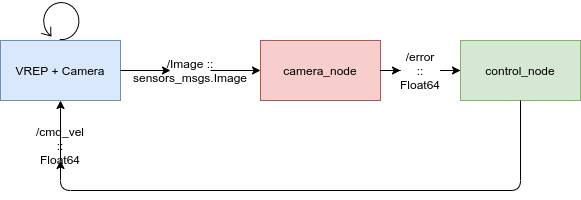
\includegraphics[scale=0.5]{Images/graph_node_simulation.png}
    \end{center}
    \caption{Graph node of the simulation}
    \label{fig:graph_node_simulation}

\end{figure}

As it is explained on the figure \ref{fig:graph_node_simulation}. The VREP camera send a through a topic \texttt{image}, a picture of the front of the car. 
Then the \texttt{camera\_node} subscriber process the image with OpenCV and return the position
of the barycenter of the line (red in the figure \ref{fig:command_explanation}), then it compute an error, we want the barycenter of line in the middle of the windows, as it's shown on figure \ref{fig:command_explanation}. 
This error is sent through a topic \texttt{error}, the controller is suscribed to this topic,
it generate a command thanks to a PD command law which is sent to VREP. And now the car can loop forever, and achieve 
the perfect run in 1'15'' ! 🚙 🏁 🕙

\subsection{Regulation}
\begin{figure}[ht!]
    \begin{center}
        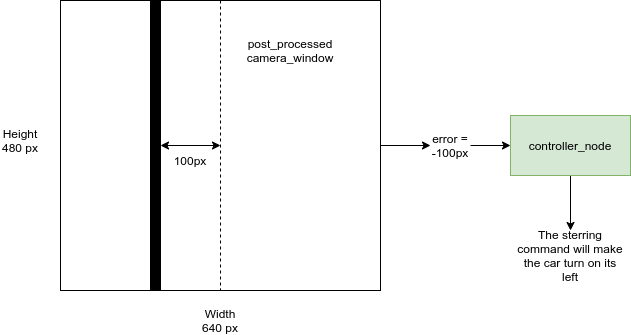
\includegraphics[scale=0.5]{Images/command_explanation.png}
    \end{center}
    \caption{Explanation of the command : line in black, barycenter in red}
    \label{fig:command_explanation}

\end{figure}
We implemented a PD regulation. Let's call $(c_x, (c_y)$, the barycenter of white line, the car is required to stay in the middle of the line.
Therefor we compute an error : $e = (width/2 - c_x) + (height/2 - c_y)$ and then the command u equals : 
$u = K_p e + K_d \frac{de}{dt}$. This command is computed in the controller and sent to vrep.


The result in video : \footnote{\url{https://www.youtube.com/watch?time_continue=10&v=_vIXo1TvG0w&feature=emb_logo} ⏯}  




